\documentclass[titlepage, a4paper, 12pt, reqno, openany]{report}
%\documentclass[12pt]{report}
%\documentclass[titlepage, a4paper, 12pt, reqno, openany]{article}
%\documentclass[12pt]{article}
%%%%%%%%%%%%%%%%%%%%%%%%%%%%%%%%%%%%%%%%%%%%%%%%%%%%%%%%%%%%%%%%%%%%%%%%%%%%%
\usepackage{titlepic}
%%%%%%encoding%%%%%%
\usepackage[T1]{fontenc}
\usepackage[utf8]{inputenc}
\usepackage{hyphenat}
\usepackage[portuguese]{babel}
%%%%%%Hyphenation rules%%%%%%
\usepackage{graphicx} %permite inserir figuras
\usepackage[font=small,labelfont=bf]{caption} %reference figures
%\usepackage{subcaption}
\usepackage{color,colortbl,multirow}
\usepackage[top=2cm,left=1cm,right=1cm,bottom=2cm]{geometry}
%\usepackage[margin=2cm]{geometry} %margens
%\usepackage[left=2cm,top=1cm,bottom=2cm,right=3cm,nohead,nofoot]{geometry}
\usepackage{paralist}
\usepackage{float}
\usepackage{verbatim}
\usepackage{lipsum}
\usepackage{multicol}
\usepackage{babelbib}
\usepackage{amsfonts}
\usepackage{amsmath}
\usepackage{amssymb}
%%%%%%%%%%%%%%%%%%%%%%%%%%%%%%%%%%%%%%%%%%%%%%%%%%%%%%%%%%%%%%%%%%%%%%%%%%%%%%%
\usepackage[usenames,dvipsnames,svgnames,table]{xcolor} %\usepackage[usenames]{color} %permite letras coloridas
\usepackage{adjustbox}
\usepackage{makecell}
%\usepackage{times}
%\usepackage{makeidx} %para criar índice remissivo
%\usepackage{array}
%\usepackage{supertabular}
%\usepackage{bm}
%\usepackage{booktabs}
%\usepackage{boxedminipage}
%\usepackage{caption}
%\usepackage{changepage}
%\usepackage{cite}
%\usepackage{easylist}
%\usepackage{esint}
%\usepackage{eucal}
%\usepackage{fancyhdr}
%\usepackage{hyperref} %index dentro de red boxes
%\usepackage{indentfirst}
%\usepackage{latexsym}
%\usepackage{listings}
%\usepackage{mathptmx}
%\usepackage{mathrsfs} %permite o uso de letras trabalhadas
%\usepackage{microtype}
%\usepackage[normalem]{ulem} %permite sublinhar palavras
%\usepackage{pifont}
%\usepackage{rotating}
%\usepackage{setspace}
%\usepackage{syntonly} %speedup work desabling pdf converse \syntaxonly
%\usepackage{subfiles}
%\usepackage{textcomp}
%\usepackage{theorem}
%\usepackage{ulem}
%\usepackage{url}
%\usepackage{wrapfig}
%%%%%recent%%%%%
%\usepackage{cancel}
%\usepackage[fleqn]{mathtools}
%\usepackage{pdfpages}
%\usepackage{pdflscape}
%\usepackage{todonotes}
%\usepackage{siunitx}
%%%%%%%%%%%%%%%%%%%%%%%%%%%%%%%%%%%%%%%%%%%%%%%%%%%%%%%%%%%%%%%%%%%%%%%%%%%%%%%%%%%
%\renewcommand\thesection{\arabic{section}}
%\renewcommand\thesubsection{\thesection.\arabic{subsection}}
%%%%%%%%%%%%%%%%%%%%%%%%%%%%%%%%%%%%%%%%%%%%%%%%%%%%%%%%%%%%%%%%%%%%%%%%%%%%%%%%%%%%
\begin{comment}
\usepackage{enumitem}
\setlistdepth{12}
\newlist{enumitem}{enumerate}{12}
\setlist[enumitem,1]{label=\roman*)}
\setlist[enumitem,2]{label=\alph*)}
\setlist[enumitem,3]{label=\arabic*)}
\setlist[enumitem,4]{label=(\roman*)}
\setlist[enumitem,5]{label=(\alph*)}
\setlist[enumitem,6]{label=(\arabic*)}
\setlist[enumitem,7]{label=\roman*)}
\setlist[enumitem,8]{label=\alph*)}
\setlist[enumitem,9]{label=\arabic*)}
\setlist[enumitem,10]{label=(\roman*)}
\setlist[enumitem,11]{label=(\alph*)}
\setlist[enumitem,12]{label=(\arabic*)}
\end{comment}

%%%%%%%%%%%%%%%%%%%%%%%%%%%%%%%%%%%%%%%%%%%%%%%%%%%%%%%%%%%%%%%%%%%%%%%%%%%%%%%%%%%%
\begin{comment}
\usepackage{enumerate}
\renewcommand{\labelitemi}{$\bullet$}
\renewcommand{\labelitemii}{$\cdot$}
\renewcommand{\labelitemiii}{$\diamond$}
\renewcommand{\labelitemiv}{$\ast$}
\end{comment}

%%%%%%%%%%%%%%%%%%%%%%%%%%%%%%%%%%%%%%%%%%%%%%%%%%%%%%%%%%%%%%%%%%%%%%%%%%%%%%%%%%%%
\begin{comment}
\usepackage{tikz}
\usepackage{circuitikz}
\usetikzlibrary{matrix,shapes.geometric,arrows,trees,positioning,calc}
%%%%%%%%%%%%%%%%%%%%%%%pre defined figures%%%%%%%%%%%%%%%%%%%%%
\tikzstyle{RECTANGLE_2} = [rectangle, draw, text width=5em, text centered, rounded corners, minimum height=4em]
\tikzstyle{RECTANGLE_3} = [rectangle, rounded corners, minimum width=3cm, minimum height=1cm,text centered, draw=black, fill=red!80]
\tikzstyle{RECTANGLE_4} = [rectangle, draw, fill=blue!20, text width=3cm, text centered, minimum height=4em]
\tikzstyle{RECTANGLE_5} = [rectangle, minimum width=3cm, minimum height=1cm, text centered, text width=3cm]
\tikzstyle{RECTANGLE_6} = [rectangle, draw, fill=blue!20, text width=5em, text centered, rounded corners, minimum height=4em]
\tikzstyle{RECTANGLE_7} = [rectangle, draw, fill=blue!20, text width=5em, text centered, rounded corners, minimum height=4em]
\tikzstyle{RECTANGLE_8} = [rectangle, draw, align=left, fill=blue!20]
\tikzstyle{RECTANGLE_1} = [rectangle, rounded corners, minimum width=1cm, minimum height=1cm,text centered, draw=black, fill=green!%30]
\tikzstyle{DIAMOND_1} = [diamond, draw, fill=blue!20, text width=4.5em, text badly centered, node distance=4cm, inner sep=0pt]
\tikzstyle{DIAMOND_2} = [diamond, minimum width=3cm, minimum height=1cm, text centered, draw=black, fill=green!30]
\tikzstyle{DIAMOND_3} = [diamond, draw, text width=4.5em, text badly centered, node distance=3cm, inner sep=0pt]
\tikzstyle{DIAMOND_4} = [diamond, draw, fill=blue!20, text width=4.5em, text badly centered, node distance=3cm, inner sep=0pt]
\tikzstyle{DIAMOND_5} = [diamond, draw, fill=blue!20, text width=4.5em, text badly centered, node distance=3cm, inner sep=0pt]
\tikzstyle{DIAMOND_6} = [diamond, draw, fill=blue!20, text width=4.5em, text badly centered, node distance=4cm, inner sep=0pt]
\tikzstyle{DIAMOND_7} = [diamond, draw, align=left, fill=blue!20]
\tikzstyle{ELLIPSE_1} = [draw, ellipse,fill=red!20, node distance=3cm, minimum height=2em]
\tikzstyle{ELLIPSE_2} = [draw, ellipse,fill=red!20, node distance=3cm, minimum height=2em]
\tikzstyle{ELLIPSE} = [draw, ellipse,fill=red!20, node distance=3cm, minimum height=2em]
\tikzstyle{TRAPEZIUM_1} = [trapezium,trapezium left angle=70,trapezium right angle=-70,minimum height=0.6cm, draw, fill=blue!20, text width=4.5em, text badly centered, node distance=3cm, inner sep=0pt]
\tikzstyle{TRAPEZIUM_2} = [trapezium, trapezium left angle=70, trapezium right angle=110, minimum width=3cm, minimum height=1cm, text centered, draw=black, fill=blue!30]
\tikzstyle{TRAPEZIUM_3} = [trapezium,trapezium left angle=70,trapezium right angle=-70,minimum height=0.6cm, draw, fill=blue!20, text width=4.5em, text badly centered, node distance=3cm, inner sep=0pt]
\tikzstyle{ARROW} = [thick,->,>=stealth]
\tikzstyle{LINE} = [draw, -latex']
\tikzstyle{MYLINE} = [draw, ->,  thick, shorten <=4pt, shorten >=4pt]
\tikzstyle{TEXT_1}=[draw,text centered,minimum size=6em,text width=5.25cm,text height=0.34cm]
\tikzstyle{TEXT_2}=[draw,text centered,minimum size=2em,text width=2.75cm,text height=0.34cm]
\tikzstyle{TEXT_3}=[draw,minimum size=2.5em,text centered,text width=3.5cm]
\tikzstyle{TEXT_4}=[draw,minimum size=3em,text centered,text width=6.cm]
\tikzstyle{CIRCLE_1}=[draw,shape=circle,inner sep=2pt,text centered, node distance=3.5cm]
\tikzstyle{CIRCLE_2}=[draw,shape=circle,inner sep=4pt,text centered, node distance=3.cm]
\end{comment}

%%%%%%%%%%%%%%%%%%%%%%%%%%%%%%%%%Not Adviced%%%%%%%%%%%%%%%%%%%%%%%%%%%%%%%%%%%%%%%%
%\usepackage{showidx} %for troubleshooting index
%\usepackage{showkeys} %for troubleshooting \label \ref
%\usepackage{pxfonts}

%%%%%%%%%%%%%%%%%%%%%%%%%%%%%%%%%claching Package%%%%%%%%%%%%%%%%%%%%%%%%%%%%%%%%%%%
%\usepackage{pgfplots}
%\usepackage{natbib}
%\usepackage[usenames]{color} %permite letras coloridas
%\usepackage{xypic}

%%%%%%%%%%%%%%%%%%%%%%%%%%%%%%%%%Not Installed Yet%%%%%%%%%%%%%%%%%%%%%%%%%%%%%%%%%%

%%%%%%%%%%%%%%%%%%%%%%%%%%%%%%%Com Dependencias%%%%%%%%%%%%%%%%%%%%%%%%%%%%%%%%%%%%%
%\usepackage{glossaries}
%\usepackage[version=3]{mhchem}

%%%%%%%%%%%%%%%%%%%%%%%%%%%%%%%%%%%%%%%%%%%%%%%%%%%%%%%%%%%%%%%%%%%%%%%%%%%%%%%%%%%%
% alguns pacotes nao sao reconhecidos, ter atencao quais usar em differents computadores, tambem alguns pacotes entram em conflito.
\newtheorem{theorem}{Theorem}
\newtheorem{lemma}{Lemma}
\newtheorem{definition}{Defini\c{c}\~{a}o}
\newtheorem{notation}{Notation}

%%%%%%%%%%%%%%%%%%%%%%%%%%%%%%%%Not Working%%%%%%%%%%%%%%%%%%%%%%%%%%%%%%%%%%%%%%%%%
%\usepackage{itemize}
%\usepackage{named}
%\usepackage{amscls}
%\usepackage{fullpage}

%%%%%%%%%%%%%%%%%%%%%%%%%%%%%%%%%%%%%%%%%%%%%%%%%%%%%%%%%%%%%%%%%%%%%%%%%%%%%%%%%%%%
%\usepackage{apacite} %Bibliography style
%%%%%%%%%%%%%%%%%%%%%%%%%%%%%%%%%%%%%%%%%%%%%%%%%%%%%%%%%%%%%%%%%%%%%%%%%%%%%%%%%%%%
\makeindex
%%%%%%%%%%%%%%%%%%%%%%%%%%%%%%%%%%%%%%%%%%%%%%%%%%%%%%%%%%%%%%%%%%%%%%%%%%%%%%%%%%%%
\begin{document}
%\bibliographystyle{apacite}
\bibliographystyle{babplain}
%%%%%%%%%%%%%%%%%%%%%%%%FIX SECTION NUMBERING IN CASE REPORT%%%%%%%%%%%%%%%%%%%%%%%%
\renewcommand\thesection{\arabic{section}}
\renewcommand\thesubsection{\thesection.\arabic{subsection}}
\renewcommand\thesubsubsection{\thesection.\thesubsection.\arabic{subsubsection}}

\begin{minipage}{\linewidth}

\title{Comportamento Organizacional}
\author{
\emph{S\'{e}rgio Santos},\;$N^o$:\; 1020881 \\
\emph{Nome 2},\;$N^o$:\; 2000000\\
\emph{Nome 3},\;$N^o$:\; 3000000\\
%\emph{Nome 4},\;$N^o$:\; 4000000\\
%\emph{Nome 5},\;$N^o$:\; 5000000\\
}
\date{\today}
%\titlepic{
\includegraphics[scale=0.50]{./image/ROQ/ROQ.jpg}}

\begin{titlepage}
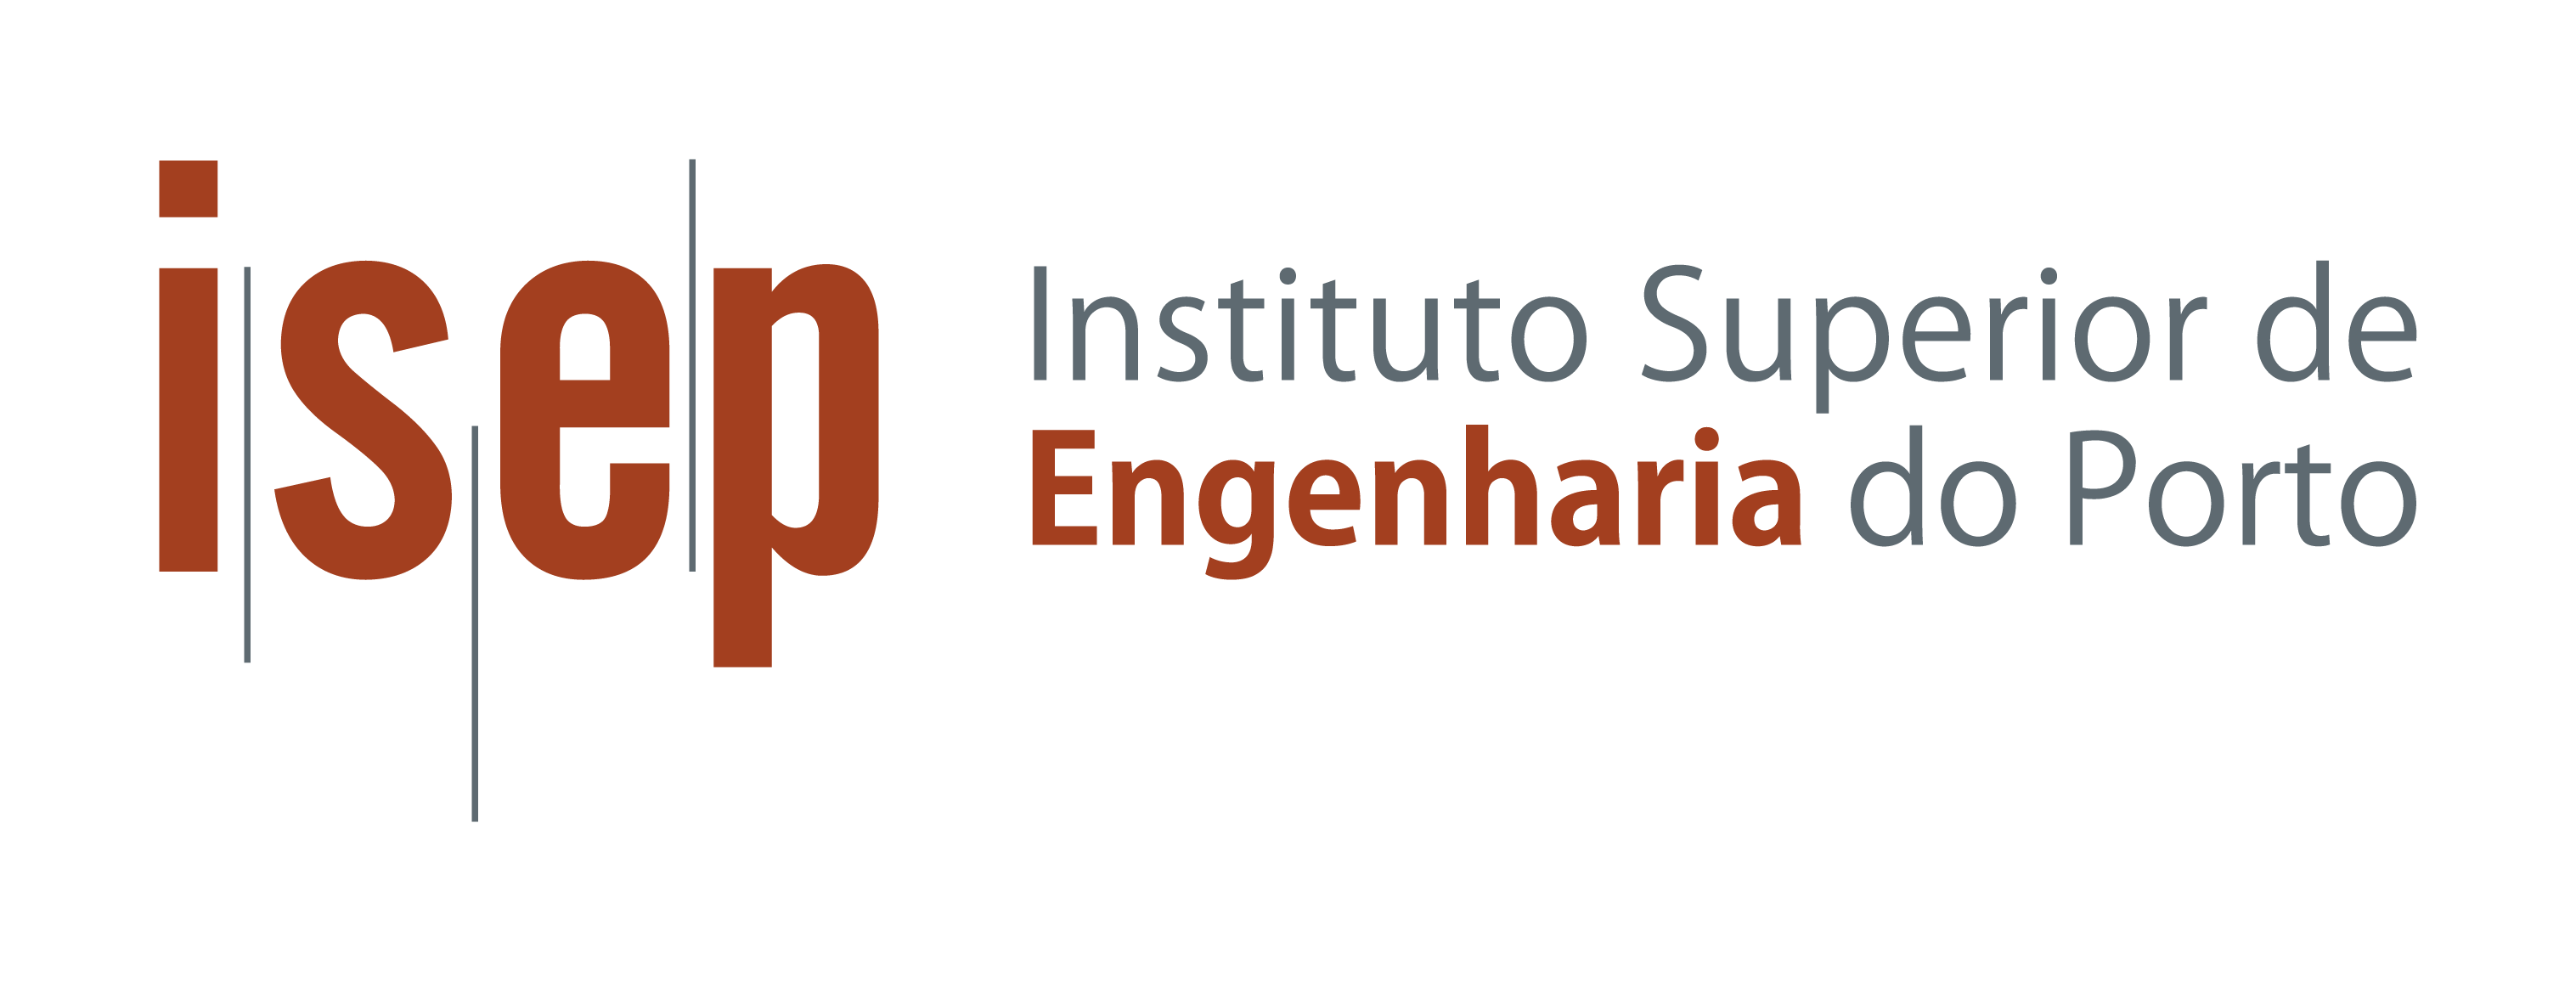
\includegraphics[scale=0.60]{./image/capa/ISEP_marca_cor_grande.png}
\maketitle
\vspace{8cm}
\begin{flushleft}

\includegraphics[scale=0.50]{./image/ROQ/ROQ.jpg}
\end{flushleft}
\end{titlepage}

\end{minipage}

\tableofcontents
%\appendix
\pagestyle{plain} %plain headings empty
%\setcounter{chapter}{0}
%\numberwithin{page}{section}
%\renewcommand{\abstractname}{Executive Summary}
\setlength{\parindent}{0in}
%%%%%%%%%%%%%%%%%%%%%%%%%%%%%%%%%%%%%%%%%%%%%%%%%%%%%%%%%%%%%%%%%%%%%%%%%%%%%%%%%%%%%%%%%%%%%%%%%%%
\newpage
\label{Resumo}
\begin{abstract}
Este trabalho consiste na análise de uma organização, onde vai ser feito sua descrição e um diagnostico da \textcolor{blue}{Cultura Organizacional} aplicando o modelo de \textcolor{blue}{Ogbonna \& Harris} e feito uma reflexão do seu impacto na organização e nos colaboradores.\\


A Cultura Organizacional é fundamental para as organizações poder evoluir e atingir seus objetivos com sucesso. O estudo da cultura presente na organização e a forma de à moldar para melhor servir a sociedade e mercado sera abordado neste relatório.\\
\\
\\
\\
\\
\\
\textbf{Palavras Chave:} Comportamento Organizacional, Cultura Organizacional, Comunicação, Motivação, Tomada de Decisão, Liderança, Planeamento, Organização, Controlo, Improvisação Organizacional.
\end{abstract}
%%%%%%%%%%%%%%%%%%%%%%%%%%%%%%%%%%%%%%%%%%%%%%%%%%%%%%%%%%%%%%%%%%%%%%%%%%%%%%%%%%%%%%%%%%%%%%%%%%%
\newpage
\section{Introdução}
\qquad A Empresa que vai ser abordada é a {\textcolor{blue}{S.Roque ou ROQ}\\
\\
Localizada no coração do Vale do Ave, a S.Roque - Máquinas e Tecnologia Laser S.A., labora em instalações próprias com uma área coberta de aproximadamente 25.000 $m^{2}$. A empresa orgulha-se de ser hoje uma experiente e bem-sucedida PME, tendo sido distinguida pelo IAPMEI como PME Líder e de Excelência pelo quarto ano consecutivo.\\\
\\
Líder nacional no seu campo de atividade – fabrico de máquinas e equipamentos para as indústrias de estamparia têxtil e embalagem - emprega atualmente mais de 350 funcionários distribuídos pelos seus diferentes departamentos.\\
\\
Com instalações funcionais e com profissionais qualificados e experientes, a S.Roque dispõe das mais avançadas ferramentas e tecnologias na área da metalomecânica, do design e da elaboração de produto. Os equipamentos fabricados são de conceção própria, desenhados por um departamento técnico altamente especializado para corresponder aos desígnios de projeto e com o objetivo de satisfazer qualitativamente as solicitações do cliente mais exigente.\\
\\
Hoje, após a conquista e solidificação incontestável da liderança do mercado português, tornando-se num dos líderes mundiais na área da estamparia e da embalagem, a S.Roque produz e comercializa um extenso catálogo com diferentes produtos e trabalha com clientes/parceiros um pouco em todo o mundo: Espanha, França, Itália, Inglaterra, Alemanha, Holanda, Suécia, Romênia, África do Sul, Marrocos, Tunísia, Angola, Turquia, Kuwait, Índia, China, Vietnam, Malásia, Camboja, Rússia, Bulgária, Brasil, Argentina, Peru, Colômbia, Honduras, El Salvador e E.U.A.
\begin{figure}[ht]
\begin{center}
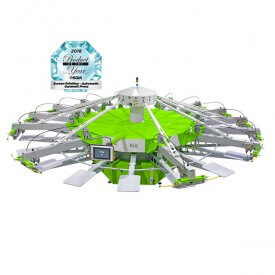
\includegraphics[scale=0.5]{"./image/ROQ/maquinas/ECO-P18_600x600-2-275x275.jpg"}
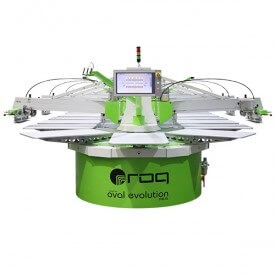
\includegraphics[scale=0.5]{"./image/ROQ/maquinas/EVO-600x600-275x275.jpg"}
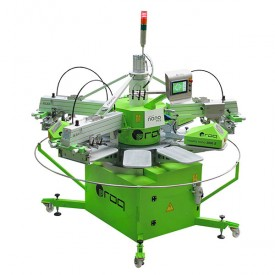
\includegraphics[scale=0.5]{"./image/ROQ/maquinas/nanop10-275x275.jpg"}
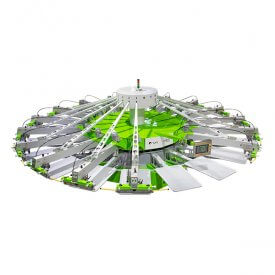
\includegraphics[scale=0.5]{"./image/ROQ/maquinas/NEXTP18-600x6001-275x275.jpg"}
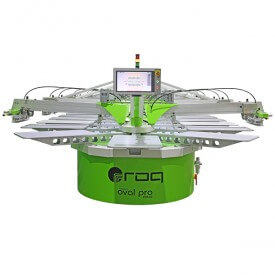
\includegraphics[scale=0.5]{"./image/ROQ/maquinas/PRO-600x600-275x275.jpg"}
\includegraphics[scale=0.5]{"./image/ROQ/maquinas/You-600x600-275x275"}
\end{center}
\caption{Produtos Principais}
\end{figure}
\\
\newpage
A S.Roque dedica-se à construção e comercialização de máquinas de estamparia têxtil há mais de 30 anos. Embora a sua génese esteja ligada à manutenção destes equipamentos, rapidamente foi identificada a oportunidade de construir de raiz este tipo de máquina. Os têxteis estavam em alta no Vale do Ave, e a S.Roque aproveitou para criar um produto de qualidade para uma clientela extremamente exigente. A empresa não se contentou em servir apenas o seu nicho de mercado, desde muito cedo que procurou a internacionalização. Numa primeira fase e por motivos geográficos criou parecerias europeias, numa segunda fase e por questões culturais dedicou-se ao Brasil e América do Sul. Neste milénio tornou-se numa marca global de referência na área onde atua. Todo e qualquer mercado está ao nosso alcance.\\
Hoje mais do que nunca não chega ter o melhor produto do mercado, é também necessário apresentar um serviço excelente e acessível em qualquer ponto do globo. A S.Roque orgulha-se de procurar a excelência em tudo em que se envolve com especial destaque para a procura de soluções.\\
\\
Em 2015 a marca S.Roque transformou-se em ROQ. Atendendo às necessidades do seculo XXI reconhecemos a necessidade de criar uma marca verdadeiramente global que consiga de uma forma eficaz transmitir mais de 30 anos de história, inovação, internacionalização e conhecimento.

%%%%%%%%%%%%%%%%%%%%%%%%%%%%%%%%%%%%%%%%%%%%%%%%%%%%%%%%%%%%%%%%%%%%%%%%%%%%%%%%%%%%%%%%%%%%%%%%%%%
\newpage
\section{Revisão da Literatura}
\qquad A disciplina \textcolor{blue}{Comportamento Organizacional} é uma ciência aplicada ao comportamento que é retirada de contribuições de disciplinas que estudam o comportamento, especificamente da psicologia e psicologia social, sociologia e antropologia.
As contribuições da psicologia são concentrada no individuo ou analise a nível micro, enquanto as outras disciplinas contribuíram para perceber a nível macro conceitos como procedimentos de grupo e organização.\\
\\
Quadro das Contribuições para o estudo desta disciplina:
\begin{figure}[H]
\centering
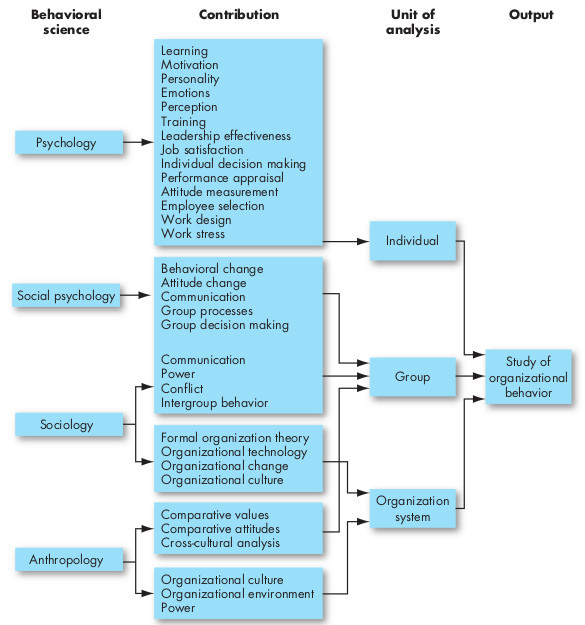
\includegraphics[scale=0.52]{./image/OB/OB_contributions.jpg}
\caption{Contribuições para OB}
\end{figure}
Este relatório esta focado no estudo da \textcolor{blue}{\textbf{Cultura Organizacional}}, portanto vou começar por definir o que é uma organização e seus objetivos.\\

Uma organização é um grupo estruturado de pessoas, um grupo onde cada pessoa é responsável por tarefas bem definidas e onde existe um sistema de articulação entre elas, que desenvolve um conjunto de atividades visando a definição e prossecução de objetivos comuns (de forma continuada no tempo).\\

O objetivo das organizações é para criar valor para os seus clientes/utentes, para os detentores do seu capital, para os seus colaboradores, para os seus fornecedores e para a sociedade em geral.\\
\newpage
Todas as organizações estão inseridas num contexto Cultural que pertence ao País ou Região e pelo modelo criado por \textit{Geer Hofstede}, Portugal tem esta distribuição nas suas dimensões:
\begin{figure}[H]
\begin{minipage}{0.3\linewidth}
\flushleft
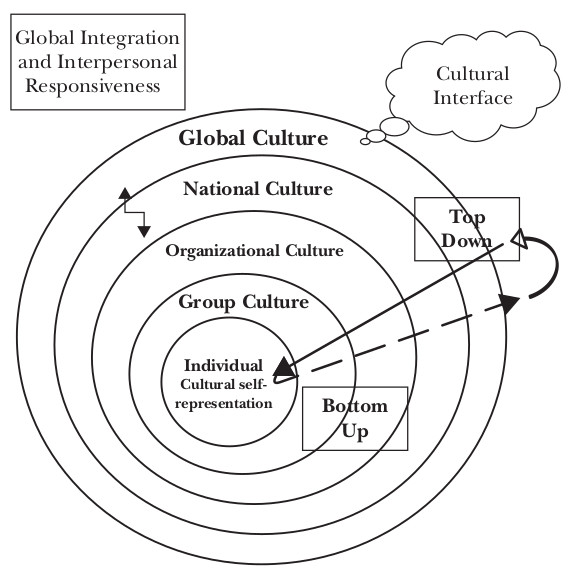
\includegraphics[scale=0.30]{./image/OB/OB_MUltilevelmodelCulture.jpg}
\end{minipage}
\hspace{1cm}
\begin{minipage}{0.4\linewidth}
\flushleft
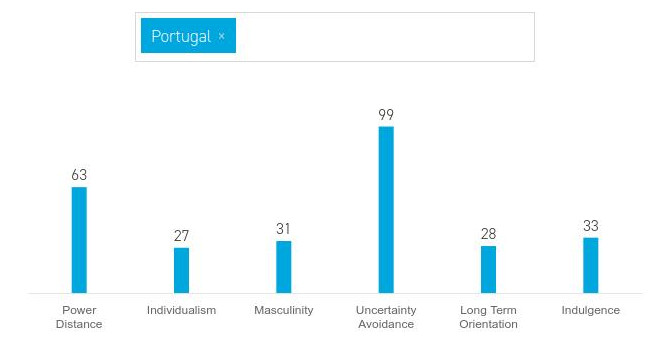
\includegraphics[scale=0.44]{./image/OB/Hofstede_pt}
\end{minipage}
\caption{Modelo de Multi-níveis da cultura e Modelo Hofstede, Portugal}
\end{figure}
Website:\\
\textit{\textcolor{green}{https://hi.hofstede-insights.com/national-culture}} \\

Ambos a Cultura da Organização e o Comportamento da Liderança foram identificados como determinantes criticos para a eficacia da organização, que se deve adaptar ao contexto transacional e externo à organização.\\

A Cultura Organizacional é um conjunto de valores, crenças e suposições partilhadas pelos membros de uma organização que a distingue das outras organizações, por exemplo, rituais e cerimonias, a historia da organização, sua estrutura e seus princípios.\\

A forma das organizações se identificarem e destacarem-se no mercado a sua cultura é expondo a sua \textcolor{blue}{Missão}, \textcolor{blue}{Visão} e seus \textcolor{blue}{Valores}.\\

A missão é os objetivos na qual a organização pretende atingir, a visão aonde pretendem chegar (futuro) e seus valores, que são suas crenças e princípios na qual defendem, e mantêm a organização unida. Como vimos anteriormente pelo estudo de \textit{Geer Hofsteed} os valores são dependente das culturas.\\

As Organizações podem ter diferentes características, e o \textcolor{blue}{\textbf{Modelo de Ogbonna \& Harris}}, carateriza a cultura das organizações em \textcolor{orange}{quatro} tipos, que pode ser análoga a outros tais como o \textbf{Modelo de Handy} e \textbf{Modelo Cameron \& Quin}.\\
\begin{figure}[H]
\flushleft
\captionsetup{justification=raggedright,singlelinecheck=false}
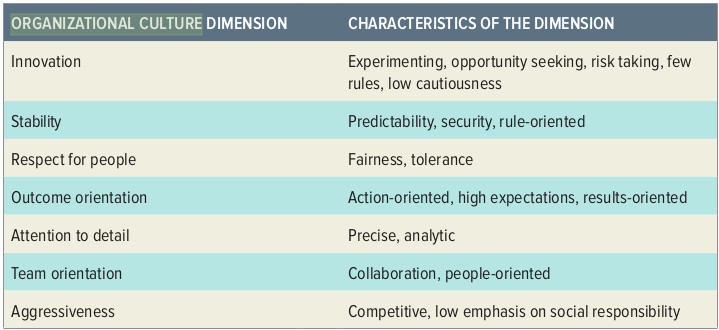
\includegraphics[scale=0.4]{./image/OB/OC_Dimensions.jpg}
\caption{Dimensões da Cultura Organizacional}
\end{figure}







\begin{comment}
Usando o método Socrático podemos perguntar qual a melhor ou melhores culturas organizacional que se enquadra na nacional nos vários tipos de organizações existentes.\\

Para criar uma cultura na organização deve-se definir uma missão, valores, visão e os objetivos.\\

Durante muito tempo tem havido estudos para descobrir a formula mágica que leva as organizações a ter sucesso, existe muitas abordagens com diferentes perspectivas, algumas convergem e outras divergem, e assim foram criados novos conceitos de forma a encapsular estilos e tipos de forma a poder se identificar quais são os mais propícios a ter uma maior elevada taxa de sucesso, conceitos tais como comportamento organizacional, cultura organizacional, performance organizacional, etc.\\
GENDER:
Nearly half of the U.S. workforce is now made up of women, and women are a growing percentage of the workforce in most countries throughout the world. Organizations need to ensure that hiring and employment policies create equal access and opportunities to individuals, regardless of gender.
RACE:
The percentage of Hispanics, blacks, and Asians in the U.S. workforce continues to increase. Organizations need to ensure that policies provide equal access and opportunities, regardless of race.
NATIONAL ORIGIN:
A growing percentage of U.S. workers are immigrants or come from homes where English is not the primary language spoken. Because employers in the United States have the right to demand that English be spoken at the workplace during job-related activities, communication problems can occur when employees’ English language skills are weak.
AGE:
The U.S. workforce is aging, and recent polls indicate that an increasing percentage of employees expect to work past the traditional retirement age of 65. Organizations cannot discriminate on the basis of age and need to make accommodations for the needs of older workers.
DISABILITY:
Organizations need to ensure that jobs and workplaces are accessible to the mentally, physically, and health challenged.
DOMESTIC PARTNERS
An increasing number of gay and lesbian employees, as well as employees with live-in partners of the opposite sex, are demanding the same rights and benefits for their partners that organizations have provided for traditional married couples.
RELIGION:
Organizations need to be sensitive to the customs, rituals, and holidays, as well as the appearance and attire, of individuals of non-Christian faiths such as Judaism, Islam, Hinduism, Buddhism, and Sikhism, and ensure that these individuals suffer no adverse impact as a result of their appearance or practices.
Tipos de descriminação:
sexual, intimidação, insultos e coerção, exclusão, incivilidade.
A satisfação melhora o desempenho.
\end{comment}
\newpage
\section{Organização}
\qquad A S.Roque é uma organização privada com fins lucrativos, que tem de oferecer valor aos seus (potenciais) clientes, aos detentores do seu capital, aos trabalhadores e aos fornecedores, existe um forte estimulo do mercado (e da concorrência) estabelece objetivos bem definidos e socialmente apetecidos para poder sobreviver e prosperar.\\
\\
A S.Roque tem uma hierarquia achatada com vários departamentos de suporte e produtivo, tem um leque de produtos (maquinas) da areá têxtil dedicado a estampagem que são la desenvolvidos e montados, isto constituí a sua atividade principal, presta serviços aos seus produtos, e também serve de apoio a outras empresas que recorrem aos seus serviços sectoriais da produção (outsourcing) para executar tarefas por encomenda, como a Roque Lazer e Serralharia (ex: Corte a laser (chapas), quinadeira, soldadura, etc)\\
\\
Sendo uma Organização Internacional tem uma equipa de Marketing e de Vendas eficaz.\\
\\
O sector produtivo tem uma implementação por produto com uma divisão de trabalho na qual é eficiente, tendo um bom controlo da qualidade.\\
\\
Hoje em dia nenhuma Organização vive em ambiente estável, e tem que estar sempre a analisar o mercado externo e estar sempre em constante adaptação ao mercado exigente, como a S.Roque tem vindo a fazer recorrendo ao mercado externo ao pais e criando novos produtos com procura competitiva. É uma empresa inovadora procura sempre aperfeiçoar seus produtos e utilizando as ferramentas mais recentes tais como o \textbf{Solid Works}.\\







\begin{comment}
Nas empresas publicas, o estimulo é sentido em menor grau ou não existente, consoante o tipo e características concretas da organização.\\

Nas organizações sem fim lucrativos e/ou dependentes do estado, existe outro tipo de estimulo os interesses dos governantes, quando o estado é parceiro ou responsável pela organização, os interesses de grupos de pressão da sociedade, etc.\\

Nas organizações sem fins lucrativos os objetivos estão em permanente discusão e/ou a ser alterados, resultando uma maior indefinição sobre as atividades a desenvolver por responsáveis e por colaboradores.\\

Teoria de Geer Hofteed.\\

Best practices can come from national, say the American National Standards Institute (ANSI) or the Canadian Standards Association (CSA), or international, say ISO or Institute of Electrical and Electronics Engineers (IEEE), standards organizations, professional associa-tions, or consulting firms.\\

Eliminar desperdício e resolução de problemas.\\

Confiança na liderança e operadores.\\

Both organizational culture and a leader’s behaviors have been identified as critical determinants of an organization’s effectiveness\\

Leaders have long been viewed as a primary influence on the creation of organizational culture (e.g. Bennis and Nanus, 1985; Schein, 1983). According to Schein (1985), the “only thing of real importance that leaders do is to create and manage culture”\\

No organization today exists in a stable environment. Current scholars, especially the
proponents of complexity theories, consider that all organizations are under the influence
of multiple changes (Brown and Eisenhardt, 1997; Burnes, 2004a; Stacey et al., 2002;
Styhre, 2002; Tetenbaum, 1998). According to these scholars, change is inherent in
human action and therefore necessarily occurs in any context of human social interactions
(Ford and Ford, 1995). As organizations are sites of continuously evolving human action,
they are in a continuous state of change and, in order to survive, must develop the ability
to continuously change themselves (Burnes, 2004b; Tsoukas and Chia, 2002).\\

Constante mudança de adaptação ao meio ambiente.\\

acknowledge that even in US and European companies, success rates are
not spectacular regarding efforts to change vision, values, and culture or business systems
and processes (Beer and Nohria, 2000; Beer et al., 1990; Carr et al., 1996).\\

Característica de bons Objetivos\\
- Claros\\
- Concisos\\
- Calendarizados\\
- Atingíveis\\

Tipos de organizações\
- Organização privadas com fins lucrativos\\
- Organização privadas sem fins lucrativos\\
- Organização publicas com fins lucrativos\\
- Organização publicas sem fins lucrativos\\

tipos de hierarquias\\
tipos de departamentalizações\\
organização por processo\\

A divisão do trabalho, permitiu a redução do tempo de aprendizagem, isto é, cada um tem as suas funções, aumentando a produtividade. Cada um executa uma parte das tarefas necessárias a fabricação.\\

Gestão:\\ \\
\begin{minipage}{20cm}
\begin{minipage}{5cm}
Instrumentos
\begin{enumerate}
\item Planear
\item Organizar
\item Controlar\\ \\
\end{enumerate}
\end{minipage}
\begin{minipage}{5cm}
Funções
\begin{enumerate}
\item Liderança
\item Comunicação
\item Motivação
\item Tomada de decisão
\end{enumerate}
\end{minipage}
\end{minipage}

Cadeia de valor\\
-Atividades principais\\
-Atividades de suporte\\

Cadeia de valor da organização é a sequencia de atividades e fluxos de informação que uma organização e os seus fornecedores devem desenvolver para desenhar, produzir, oferecer, entregar e suportar os seus produtos, estas são as atividades principais.\\

As atividades de suporte são as que apoiam um bom desempenho na realização das actividades principais.\\
- atividade administrativa e financeira\\
- atividade da gestão do pessoal\\
- atividade jurídica\\
- planeamento, controlo e gestão\\
- gestão de sistemas e tecnologia\\

A atividade de suporte não contribuem diretamente para a criação do valor.\\

Atividades de suporte e principal.\\
funções da Gestão sã Instrumental, Comportamental e Estrutural.\\

Cumprir os objetivos é ser eficaz.\\

Para gerir a produção (planear, organizar, dirigir e controlar), há que recolher um elevado volume de informação de controlo, sendo frequentemente necessário refazer o planeamento.\\

- Implementação por projeto\\
- Implementação por processo\\
- Implementação por células\\
- Implementação por cadeia ou em linha\\
- Implementação por produto\\

Na implementação por célula de fabrico procura agrupar os produtos segundo a semelhança das suas rotinas operatórias.\\
Na implementação por processo, é possível cada serie (ou lote) ser processado integralmente num dado centro, antes de avançar para o centro onde irá sofrer a operação de transformação seguinte.\\
A análise ABC pode ser utilizada para averiguar quais as principais encomendas responsáveis pela sobrecarga de um dado centro de trabalho.\\

Organizar é estipular quem faz o quê, atribui-se os recursos necessários para o fazer, criar um sistema de informação para verificar execução.\\
\end{comment}
\newpage
\section{Cultura Organizacional}
\qquad Os fundadores da organização tem um grande impacto no processo de formação da cultura organizacional através da imposição das suas crenças e suposições no grupo. A adoção das crenças, valores e suposições que formam a cultura da organização é depois reforçada pelos vários comportamentos primários dos lideres.\\

\textcolor{blue}{\Large{S.Roque}}

Planeamento Estratégico:

\subsection{Missão}
\begin{comment}
A missão de uma organização consiste na sua razão de existir, actual e futura.\\
\end{comment}
A S.Roque tem como missão a constante inovação e criação de produtos de excelência na área da estamparia têxtil à peça. Para tal, aposta em múltiplos vetores complementares: tecnologia, qualidade e recursos humanos especializados. Estimula de forma persistente a sua veia empreendedora e internacional, promovendo para isso o contínuo aperfeiçoamento do seu serviço, em qualquer parte do mundo, mantendo-se fiel aos princípios éticos e de sustentabilidade.

\subsection{Visão}
Trilhar um percurso sustentável de inovação, de expansão internacional, de excelência em todas as soluções que lançamos para o mercado, de qualidade absoluta, para nos mantermos como líder na nossa área de negócio.

\subsection{Valores}
\begin{itemize}
\setlength\itemsep{-0.3em}
\item Ação dentro dos princípios morais e éticos da empresa para com os seus stakeholders.
\item Atuação sempre no interesse dos nossos parceiros de forma a promover a sua satisfação e fidelização.
\item Excelência conseguida através de trabalho de equipa, competência e responsabilidade.
\item Qualidade absoluta.
\item Inovação promovida pelo ADN empreendedor da S. Roque.
\item Sustentabilidade ambiental e segurança.
\end{itemize}\par

Além da sua definição estratégica da organização pode fazer-se objetivos pelo método \textcolor{blue}{\textbf{SMART}} e uma análise \textcolor{blue}{\textbf{SWOT}}, que não é o proposito deste relatório.\\








\begin{comment}
O que lhes chama a atenção e medem; suas reações a incidentes criticos, alocação de meios, papeis assumidos, e partilha de informação; recompensas e delegaçao de poder; recrutamento, seleção e promoção. As lideranças chave tem como responsabilidade de modificar a cultura de forma a estar atualizada com as mudanças exigidas.\\

Aqui distingue-se dois tipos de lideres os transacionais e os de transfromação. “culture affects leadership  as much as leadership affects culture”

Planear é estabelecer os objetivos a atingir e o percurso de ações.\\

A formulação, avaliação e seleção de estratégias e o desenvolvimento dos planos mais detalhados para as pôr em prática são feitos após a definição da missão e da análise do meio ambiente da organização.\\

Ferramentas para avaliar o cumprimento dos objetivos\\
- benchmarking\\
- scorecard management\\
- Banco de Portugal\\

Método de demonstrar o desempenho de uma organizações através da eficacia, eficiência e seu rendimento.\\

Eficacia avalia em que medida os objetivos estão alinhados com a necessidades sociais que ela se propõe a satisfazer, ou seja, em que medida os seus objetivos são a tal adequados.\\

Eficiência avalia a economia de recursos utilizados para realizar os seus objetivos, requer uma boa estruturação dos processos seguidos nas atividades, o que leva tempo e custa dinheiro.\\

Missão - SWOT Meio Ambiente (transacional e contextual(PEST)) - Objetivos - Implementação.\\

O sucesso das empresas está correlacionada positivamente com o seu planeamento.\\

Na análise do meio ambiente transacional, analisa-se o comportamento previsional das entidades com quem a organização interage.\\

Controlo.\\
O controlo pode ser encarado como um processo de aprendizagem.\\
O controlo deve servir, acima de tudo, para ajudar a garantir que os objetivos estabelecidos são atingidos.\\
Se a informação recolhida e os resultados apurados no processo de controlo não conduzem a ações de correção quando necessário, este será não só inútil, mas até prejudicial.\\
O recurso aos sistemas de informação permite, em geral, simplificar os procedimentos de controlo.\\

Controlar é os procedimentos de verificar sua execução, estar atento a imprevistos e pronto a correções recorrendo a re-organização e/ou novo planeamento, também pode-se optar por não fazer nada.\\
\end{comment}
\newpage
\section{Estudo da Cultura Organizacional segundo o Modelo Ogbonna \& Harris}
\qquad O Modelo Ogbonna \& Harris estuda a relação entre as variáveis Estilos de liderança, Cultura organizacional e Performance organizacional. Este modelo foi derivado de um estudo empírico na Inglaterra através de os procedimentos científicos e estatísticos na analise dos dados obtidos por questionários as empresas envolvidas.\\

\subsection{Modelo Ogbonna \& Harris}
{\bf As variáveis estão abaixo descritas na qual foram consideradas no estudo.} \\

\begin{minipage}[t]{.3\linewidth}
\quad Estilos de Liderança:
\begin{itemize}
\setlength\itemsep{-0.3em}
\item Participativo
\item Orientado as pessoas
\item Orientado as tarefas
\end{itemize}
\end{minipage}
\begin{minipage}[t]{.3\linewidth}
\quad Tipos de Cultura:
\begin{itemize}
\setlength\itemsep{-0.3em}
\item Inovadora
\item Competitiva
\item Burocrática
\item Comunitária
\end{itemize}
\end{minipage}
\begin{minipage}[t]{.3\linewidth}
\quad Medição do Sucesso:
\begin{itemize}
\setlength\itemsep{-0.3em}
\item Satisfação dos Clientes
\item Taxa crescimento vendas
\item Cotação no mercado
\item Vantagens Competitivas
\item Volume de vendas
\end{itemize}
\end{minipage}
\vspace{2cm}\\

Os resultados obtidos na determinação do Estilos de liderança e tipo de Cultura Organizacional das empresas Estudadas e depois o Modelo que foi criado são mostrados nas paginas seguintes.\\

\begin{figure}[H]
\centering
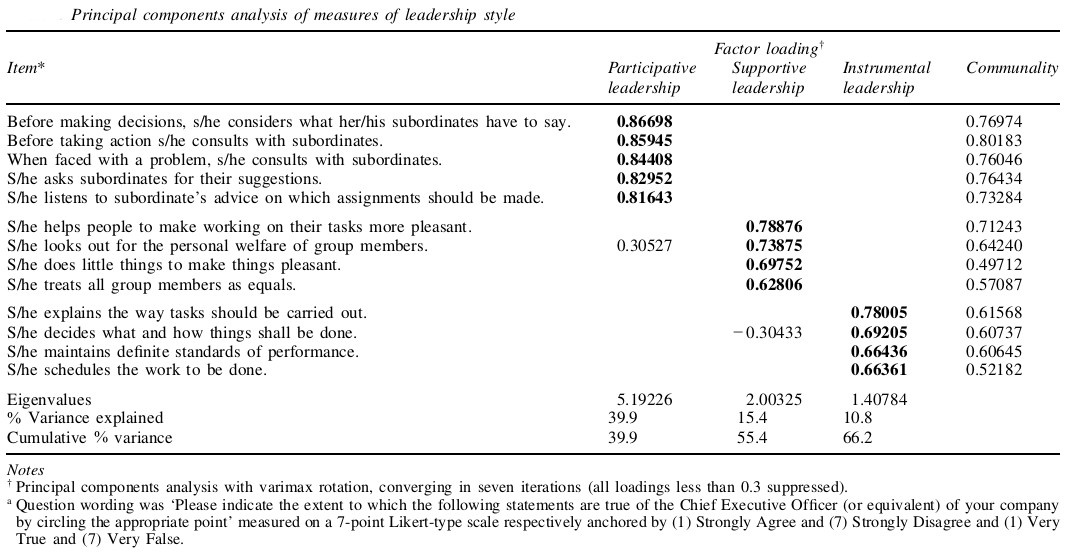
\includegraphics[scale=.5]{"./image/OB/Leadership.jpg"}\\
\caption{Estilos de Liderança}
\end{figure}\par
\vspace{1cm}
\begin{figure}[H]
\centering
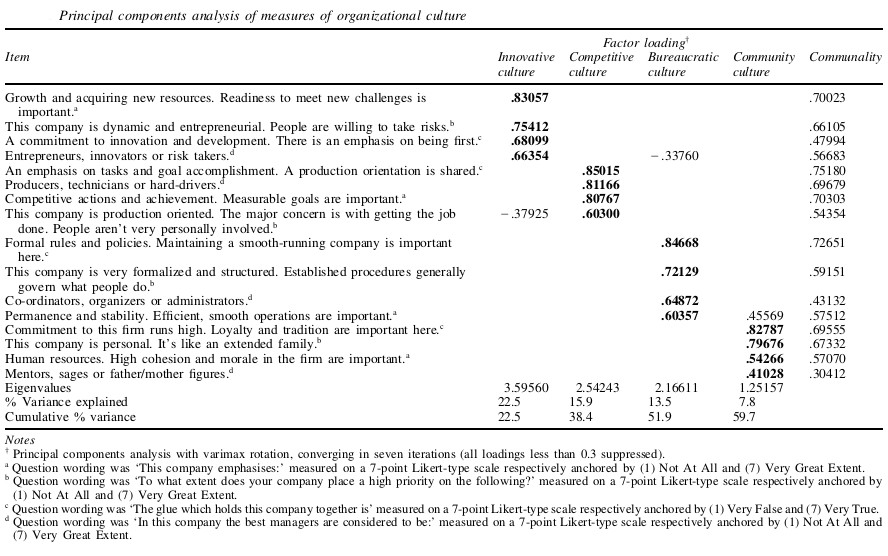
\includegraphics[scale=.6]{"./image/OB/Culture.jpg"}\\
\caption{Cultura Organizacional}
\end{figure}\par

\begin{figure}[H]
\centering
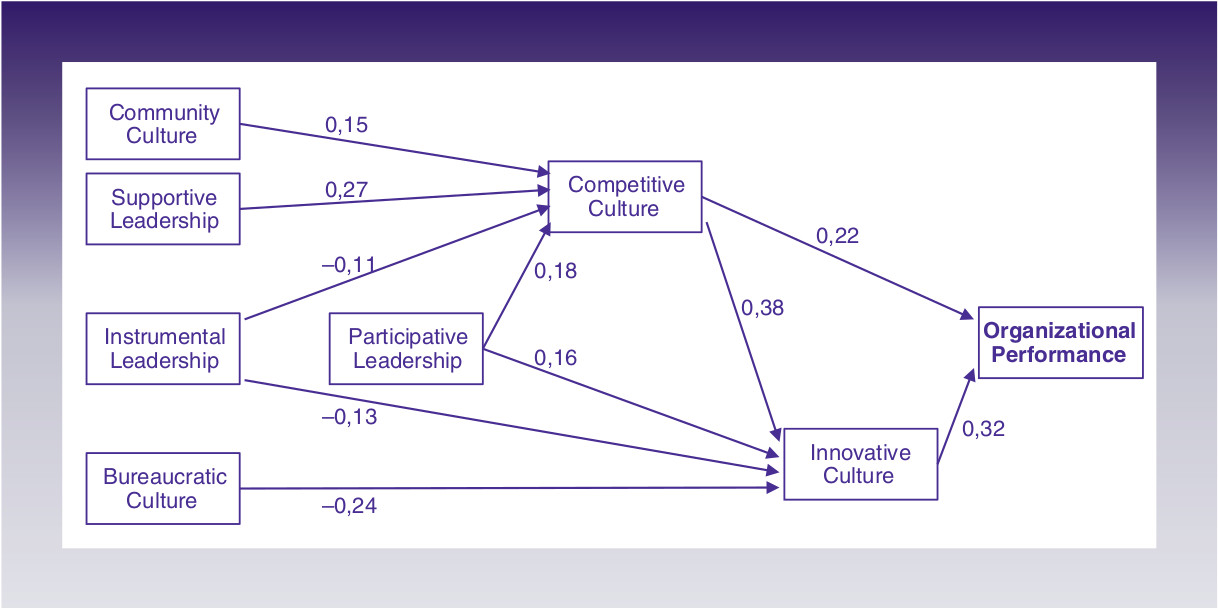
\includegraphics[scale=.35]{"./image/OB/Ogbonna & Harris.jpg"}\\
\caption{Modelo Ogbonna \& Harris}
\label{Modelo}
\end{figure}\par

\textcolor{red}{Clarificar os resultados.}\\

In their well-known and prestigious study on the relationship between leadership style , organizational culture and performance or success, Ogbonna and Harris ( 2000 ) first point out that the relationship between leadership style and success was not understood as good as the relationship between culture and success. To many practitioners that sounds weird or surprising, but at least very interesting. In their survey, in which 342 of 1000 requested English companies participated, they found that culture would actually mediate the relationship between leadership style and success. The leadership style would not be directly related to success but only indirectly. They found companies with an innovative and competitive organizational culture to be more successful than companies with a bureaucratic or a community culture. While they ascribed a more external orientation (positioning and responsiveness) to innovative and competitive cultures, they associated a rather internal orientation (integration, cohesion, uniformity) with bureaucratic or community cultures. Figure 2.6 shows the results at a glance, where the dependencies or interrelationships are quantified by means of effect factors. For companies with a bureaucratic or community culture, they could see only indirect and rather insignificant relationships between culture and success in their analyses. For companies with innovative and competitive cultures, however, they could find a strong positive and direct relationship. Thus, innovative and competitive cultures would account for nearly 25 \% of the variance in organizational performance (success). Using path analysis, they further found that only the supportive and the participative leadership style correlated positively with innovative and competitive organizational cultures. Therefore, in an innovative and competitive organizational culture, conducting a supportive and participative leadership style would be most promising to improve organizational performance or success.






\newpage
\subsection{Modelo Aplicado a S.Roque}
O Inquérito abaixo é usado para medir os componentes principais para determinar a Cultura Organizacional.
\begin{table}[h!]
\begin{adjustbox}{max width=\textwidth}
\begin{tabular}{ |c|l|c| }
\hline
\rowcolor[gray]{0.5}
Nº & Inquérito & \makecell[l]{Resp \\ 1 \; - \; 7} \\
\hline
1. & \makecell[l]{A organização preocupa-se com o crescimento e a aquisição de novos recursos, \\ e procura responder a novos desafios.} & \\
\hline
2. & \makecell[l]{A organização é dinâmica e empreendedora. \\ As pessoas estão dispostas a correr riscos.} & \\
\hline
3. & \makecell[l]{Existe um elevado empenho na inovação e no desenvolvimento. \\ Procuramos ser os primeiros.} & \\
\hline
4. & \makecell[l]{Consideram-se os melhores gestores os que são empreendedores, \\ Inovadores e tomadores de riscos.} & \\
\hline
5. & Existe uma elevada ênfase nas tarefas e no alcance de objetivos. & \\
\hline
6. & Considera-se que os melhores gestores são produtores e técnicos. & \\
\hline
7. & \makecell[l]{A organização valoriza as ações competitivas, \\ o sucesso e o alcance de objetivos mensuráveis.} & \\
\hline
8. & \makecell[l]{A organização é orientada para a produção. \\ Uma das maiores preocupações é fazer o que tem que ser feito. \\ Os empregados não estão muito envolvidos do ponto de vista pessoal.} & \\
\hline
9. & A organização valoriza muito as regras e as políticas formais. & \\
\hline
10. & \makecell[l]{A organização é muito formalizada e estruturada. \\ Os procedimentos estabelecidos orientam o que as pessoas devem fazer.} & \\
\hline
11. & Os melhores gestores são considerados os que são coordenadores ou organizadores. & \\
\hline
12. & Na organização valoriza-se a permanência, a estabilidade e a eficiência. & \\
\hline
13. & Valoriza-se muito a lealdade, a tradição e o empenhamento na organização. & \\
\hline
14. & A organização é uma espécie de grande família. & \\
\hline
15. & Valoriza-se muito a coesão e os recursos humanos. & \\
\hline
16. & \makecell[l]{Considera-se que os melhores gestores são os que atuam como mentores, \\ sábios ou figuras paternais/maternais.} & \\
\hline
\end{tabular}
\end{adjustbox}
\end{table}\par
{\tiny 1- A afirmação não se aplica rigorosamente nada à minha organização, 2- Não se aplica, 3- Aplica-se muito pouco, 4- Aplica-se alguma coisa,\\ 5- Aplica-se bastante, 6- Aplica-se muito, 7- A afirmação aplica-se completamente à minha organização
} \\
\\
\textbf{Contribuições para o Inquérito:}\\
\textbf{-} \; \textcolor{green}{Paulo Campos}\\



\textcolor{red}{Fazer tabela com resultados.}









\begin{comment}
No entanto a comparação entre os comportamentos dos lideres e as cultura organizacional, no impacto que tem na variável organização e a eficacia da liderança ainda não foram empiricamente examinados.\\
Estilos de liderança:
\begin{itemize}
\item participative leadership\\
Is gauged by the extent to which leaders allow subordinates to influence decisions by requesting input and contribution.
\item supportive leadership\\
Focuses on the degree to which the behaviour of a leader can be viewed as sympathetic, amicable, and considerate of subordinate needs
\item Instrumetal leadership\\
This measure of leadership style is akin to directive or transactional leadership and is designed to measure the extent to which leaders specify expectations, establish procedures, and allocate tasks.
\end{itemize}
Motivação teorias Moslow, Hersberg, Victor Vroom.\\
Se as condições e recompensas oferecidas aos funcionários não lhes permitirem satisfazerem algumas das suas necessidades, mais facilmente abandonam a equipa ou organização a que pertencem.\\
Motivação é o conjunto de fatores que provocam, canalizam e sustentam o comportamento das pessoas.\\
Um gestor interessado em atingir um bom desempenho estabelece objetivos atingíveis e bem defendidos.\\
Auto-confiança no desenvolvimento do trabalho pode diminuir a sua motivação.\\
Motivar é criar condições necessárias para que as pessoas se empenham na prossecução dos objetivos da organização.\\
O impacto da comunicação no desempenho da organização é muito elevado.\\
Os Gestores tem de ser coerentes e alinhados com o que transmitem de forma a criar uma estrutura de confiança.\\
Um líder de uma organização é aquele que detém capacidades de influenciar os colaboradores.\\
gestão das atividades é o exercício do poder de um gestor.\\
poder de premiar e punir é suficiente para gerir as atividades do dia a dia.\\
poder informacional.\\
Um sistema de avaliação do desempenho de uma empresa é uma valia porque é uma boa oportunidade para analisar o grau de cumprimento dos objetivos acordados.\\
A medida que as organizações se achatam, os gestores têm de aprender a permitir que os seus colaboradores tomem decisões e tenham informação sobre questões mais sensíveis.\\
Para um engenheiro é muito útil conhecer os aspectos essenciais da legislação laboral.\\
A gestão das pessoas é cada vez mais importante porque são as pessoas que têm o conhecimento e só as pessoas o podem partilhar e aplicar.\\
Numa organização, apoiar e compensar as pessoas é fundamental, mas também é indispensável falar com elas sobre os erros que cometem no sentido de serem corrigidas e evitadas no futuro.\\
Uma organização tem maior probabilidade de ter sucesso se gerir as pessoas de modo a que estas ao contribuírem para o sucesso da organização tenham também sucesso elas próprias.\\
A qualidade é a totalidade das características de um produto ou serviço, que determinam a sua aptidão para satisfazer determinadas necessidades.\\
Garantia da qualidade tem como objetivo primeiro, o controlo do processo, ou seja, a minimização ou mesmo eliminação dos erros na produção.\\
A garantia da qualidade concentra-se no controlo do processo produtivo e controlo do produto.\\
Os custos relacionados com a insatisfação dos clientes são considerados custos de não qualidade.\\
O diagrama de Pareto permite identificar rapidamente as causas vitais e as triviais de um dado problema.\\
As cartas de controlo destinam-se a detetar as variações resultantes da alteração, frequentemente de natureza aleatória e acidental, de algum dos parâmetros de processo de fabrico (ditas causas especiais).\\
As sete ferramentas clássicas da qualidade\\
- Fluxograma\\
- Registo e análise de dados\\
- Diagrama de causa - efeito (espinha de peixe 4M)\\
- Diagrama de Pareto\\
- Histogramas\\
- Diagramas de dispersão\\
- Cartas de Controlo\\
tipos de lideres\\
- Autocrático\\
- Participativo \\
- Democrático \\
- Deixa andar\\
estilo de líder\\
- Orientado as pessoas\\
- Orientado as tarefas\\
\end{comment}
\newpage
\section{Conclusões}
\qquad Nota este trabalho é fundamentado em outros autores e especialistas nas suas áreas, podendo haver erros de interpretação.\\

\textcolor{red}{Tirar as conclusões acerca da S.Roque e Comparar com o modelo Ogbona \& Harris}








\begin{comment}
The relationship between culture and leadership appears to be reciprocal—top leaders create and maintain an organizational culture, which in turn influences the values, attitudes, and behaviors of middle and entry-level leaders. Although leader–culture fit has not been specifically studied in the published literature, we believe that there is value in examining the match between a leader’s behaviors and the culture in which they work. While research hasn’t examined this at the level we discuss, current research does suggest that fit is important at the national level and at the leader–follower level. Expansion of this research will help determine what aspects of leader culture fit are determinants of leader and organizational effectiveness. Although there are a variety of approaches that researchers can take to examining leader–culture fit, we offer the following recommendations. First, although studies of perceived fit are of limited value, the ease of collecting this data should motivate researchers to start thinking about adding questions concerning leader–culture fit. Given the lack of published findings, this research can begin shaping our knowledge about this phenomenon. Second, while studies of subjective fit will be more important, researchers should utilize 360-degree measurement systems in order to also obtain the most objective fit indices possible. This practice will likely tell us more about the impact of fit than just examining leaders’ self-reports. Third, it is important to measure culture at the aggregate level in order to ensure that the actual values of the organization are being captured, not just the leader’s values. Although these recommendations may be difficult to achieve in practice, they offer the best hope of leveraging leader–culture fit for the future.\\

A actividade comportamental consiste em lidar com pessoas, comunicar instruções e receber feedback, propiciar a comunicação entre os terceiros, motivar, tomar decisões e criar condições para que os colaboradores também o possam fazer, assegurar a liderança para cumprir a execução.\\

More specifically, it suggests that culture pro-vides the normative bounds for transactional leaders to be effective and that transformational leaders influence culture through strategic decisions and vision, by celebrating success, and by identifying and rewarding employees. \\

In sum, leadership and organizational culture are related, and further, the dynamics between these constructs impact organizational effectiveness. However, the theoretical work in this area largely outweighs the empirical, and we believe there is utility in adopting a “fit” perspective for further research in this area.\\

In their meta-analysis, Kristof-Brown et al. (2005) identified five types of fit research that captured the majority of published studies: person–vocation fit, person–job fit, person–organization fit, person–group fit, and person–supervisor fit. Attempting to integrate all of these perceptions of fit, Jansen \& Kristof-Brown (2006) proposed a multidimensional theory of person–environment (PE) fit. \\

O alinhamento entre o líder e a cultura da organização influencia e sua eficacia.\\

Durante este trabalho ao enfrentar a literatura da para perceber que os estudos efetuados nas relações Liderança, cultura e eficacia são quase todos inconclusivos, apenas nos dão indicadores e em muitos casos levantam cada vez mais questões. Podemos no entanto tirar com um grau de incerteza algumas premissas como verdade e muito úteis. \\
\\
The explications of this section strongly support the thesis that the culture of an organization has a significant influence on its success. There is good reason to believe that success is promoted in the presence of an anticipatory adaptive organi- zational culture with a good portion of external orientation especially if in the mean time, a supportive and participative leadership style prevails. Culture determines, how and what we anticipate, how intensive we observe external developments or what we consider a good reason to adapt or change. Thereby, culture also influences the timing of any change. In the course of any such change ambition, culture determines the room of possibilities: What is seen as acceptable, possible, feasible, appropriate, etc.? We saw in this section that there is a strong link between the success of change projects and culture. In all of this, leaders or managers play an important role. They have to constantly assess how potential changes fi t to the cultural profile of the organization. Misjudgments cause change initiatives to suffer. If that is repeatedly the case, the success of any change project and ultimately the success of an entire organization is at danger. Therefore, it is imperative that they have suffi cient knowledge of their own organization’s culture. In order to contribute optimally to organizational success, leadership has to conduct culturally adequate behaviors, decisions and measures. At the same time, leadership has to develop the culture itself, if that has become necessary. We’ll come back to this in detail in Chap. 5 : Management of Organizational Culture on pages 245 ff. \\

These findings are broadly consistent with a range of studies which suggest that externally oriented organizational cultures are positively linked with performance (for example, Slater and Narver, 1994; Greenley, 1995) as well as a growing body of research which suggests that the alignment of organizational culture towards strategic needs is a central, albeit dificult, role for senior executives (see Harris and Ogbonna, 1999).\\

Therefore, the finding of positive associations between externally oriented cultures and performance suggests that organizational culture change efforts should focus as much on generating external focus as upon creating internal cohesion and consistency.\\
\end{comment}
\begin{comment}
A vida ensina e se não aprendemos ela insiste e persiste até morrermos.\\
A liberdade é medida pela quantidade de ética e moralidade presente na sociedade.\\
Respect is always earned never a given.\\
\end{comment}
\newpage
%%%%%%%%%%%%%%%%%%%%%%%%%%%%%%%%%%%%%%%%%%%%%%%%%%%%%%%%%%%%%%%%%%%%%%%%%%%%%%%%%%%%%%%%%%%%%%%%%%%
%\part*{Equa\c{c}\~{o}es} \label{eq}
%
\begin{flushleft}
{\bf Corrente Continua Condi\c{c}\~{o}es \index{Condi\c{c}\~{o}es} iniciais \index{iniciais} nulas \index{nulas}.}\par
\end{flushleft}
 \quad Circuito \index{Circuito} $LC$ em $C.C$:\par
%
\begin{itemize}
\item
$i(t)=\frac{V_{DC}\sqrt{LC}}{L}\quad \sin \left( \frac{t}{\sqrt{LC}}\right)\times u(t)$\par
\item
$V_L(t)=V_{DC}\quad \cos\left(\frac{t}{\sqrt{LC}} \right)\times u(t)$\par
\item
$V_c(t)=V_{DC}\quad \left(1-\cos\left(\frac{t}{\sqrt{LC}} \right) \right)\times u(t)$\par
\item
$\omega_n=\frac{1}{\sqrt{LC}}$\par
\item
$\overline{Z}=\sqrt{(\omega_n L-\frac{1}{\omega_n C})^2}$\par
\item
$\phi_p=\frac{\pi}{2}$\par
porque, $\sin(\omega_n t)= \cos(\omega_n t - \pi/2)$\par
\item
$\tau=\infty$\par
\end{itemize}
%
%%%%%%%%%%%%%%%%%%%%%
\quad Circuito \index{Circuito} $RLC$ em $C.C$:\par
%
\begin{enumerate}
%enum1
\item
Para \quad $C(C R^2-4 L)>0$ \quad (Ra\'{i}zes \index{Ra\'{i}zes} reais \index{reais} diferentes \index{diferentes}) \quad Sobreamortecido \index{Sobreamortecido}.\par
%
\begin{itemize}
\item
$i(t)=\frac{2 V_{DC} C e^{\frac{-tR}{2L}} sinh \left( \frac{t \sqrt{C(CR^2-4L)}}{2CL} \right)}{\sqrt{C(CR^2-RL)}}\times u(t)$\par
\item
$V_R(t)=R\times i(t)$\par
\item
$V_L(t)=L\dfrac{di(t)}{dt}$\par
%
\begin{minipage}{0.95\linewidth}
\makebox[\linewidth]{
\includegraphics[scale=0.75]{./Image/equacoes_1.png}
}
\end{minipage}\par
%
\item
$V_C(t)=\frac{1}{C}\int_0^ti(t)$\par
%
\begin{minipage}{0.95\linewidth}
\makebox[\linewidth]{
\includegraphics[scale=0.75]{./Image/equacoes_2.png}
}
\end{minipage}\par
%
\end{itemize}
%enum2
\item
Para \quad $C(C R^2-4 L)=0$ \quad (Ra\'{i}zes \index{Ra\'{i}zes} iguais \index{iguais})\quad Amortecimento \index{Amortecimento} cr\'{i}tico \index{cr\'{i}tico}.\par
%
\begin{itemize}
\item
$i(t)=\frac{V_{DC}}{L} \quad  t \quad e^{\frac{-R t}{2L}} \times u(t)$\par
\item
$V_R(t)=R\times i(t)$\par
\item
$V_L(t)=L\dfrac{di(t)}{dt}$\par
%
\begin{minipage}{0.95\linewidth}
\makebox[\linewidth]{
\includegraphics[scale=0.75]{./Image/equacoes_3.png}
}
\end{minipage}\par
%
\item
$V_C(t)=\frac{1}{C}\int_0^ti(t)$\par
\begin{minipage}{0.95\linewidth}
\makebox[\linewidth]{
\includegraphics[scale=0.75]{./Image/equacoes_4.png}
}
\end{minipage}\par
%
\end{itemize}
%enum3
\item
Para \quad $C(C R^2-4 L)<0$ \quad (Ra\'{i}zes \index{Ra\'{i}zes} complexas \index{complexas}) \quad Amortecido \index{Amortecido}.\par
%
\begin{itemize}
\item
$i(t)=\frac{2 V_{DC} C e^{\frac{-tR}{2L}} sin \left( \frac{t \sqrt{-C(CR^2-4L)}}{2CL} \right)}{\sqrt{-C(CR^2-4L)}}\times u(t)$\par
\item
$V_R(t)=R\times i(t)$\par
\item
$V_L(t)=L\dfrac{di(t)}{dt}$\par
%
\begin{minipage}{0.95\linewidth}
\makebox[\linewidth]{
\includegraphics[scale=0.75]{./Image/equacoes_5.png}
}
\end{minipage}\par
%
\item
$V_C(t)=\frac{1}{C}\int_0^ti(t)$\par
%
\begin{minipage}{0.95\linewidth}
\makebox[\linewidth]{
\includegraphics[scale=0.75]{./Image/equacoes_6.png}
}
\end{minipage}\par
%
\end{itemize}
\end{enumerate}
%
\begin{itemize}
\item
$| \omega_n |=\sqrt{\frac{4 L-R^2 C}{4 L^2 C}}$\par
\item
%\overrightarrow{Z}
$\overline{Z}=\sqrt{R^2 + (\omega_n L -\frac{1}{\omega_n C})^2}$\par
\item
$\phi_p=\arctan\left(\frac{\omega_n L - \frac{1}{\omega_n C}}{R}\right)$\par
\item
$\tau=\frac{2 L}{R}$\par
\end{itemize}
%%%%%%%%%%%%%%%%%%%%%%%%%%%%%%%%%%%%%%%%%%
\begin{flushleft}
{\bf Corrente \index{Corrente} Alternada condi\c{c}\~{o}es \index{Condi\c{c}\~{o}es} iniciais \index{iniciais} nulas \index{nulas}}.
\end{flushleft}
\quad Circuito \index{Circuito} $RLE$ em $C.A$:\par
\begin{itemize}
\item
$i(t)=C_T\ e^{-\frac{R}{L}t}+\frac{V_{m\acute{a}x}}{\overline{Z}}\sin(\omega t + \alpha - \phi_p)-\frac{E}{R}$\newline
$i(t)=C_T\ e^{-\frac{R}{L}t} + C_1 \cos (\omega t) + C_2 \sin(\omega t)-\frac{E}{R}$
\item
$I(\omega t)=C_T\ e^{-\frac{R}{L \omega}\omega t}+\frac{V_{m\acute{a}x}}{\overline{Z}}\sin(\omega t + \alpha - \phi_p)-\frac{E}{R}$
\item
$\overrightarrow{Z}=R+j\omega L$\\
$\overline{Z}=\sqrt{R^2 + (\omega L)^2}$
\item
$\phi_p=\arctan(\frac{\omega L}{R})$
\item
$C_T=\frac{E}{R}-\frac{V_{m\acute{a}x}}{\overline{Z}}\sin(\alpha - \phi_p)$
\item
$C_T=\frac{V_{m\acute{a}x}}{R^2 + (\omega L)^2}(L \omega \cos(\alpha) - R \sin (\alpha))+\frac{E}{R}$
\item
$C_1=\frac{V_{m\acute{a}x}}{R^2 + (\omega L)^2}(R \sin (\alpha) - L \omega \cos(\alpha))$
\item
$C_2=\frac{V_{m\acute{a}x}}{R^2 + (\omega L)^2}(R \cos (\alpha) + L \omega \sin (\alpha))$
%
\end{itemize}
%%%%%%%%%%%%%%%%%%%%%%%
%\part*{Defini\c{c}\~{o}es} \label{def}
\begin{definition}
Capacit\^{a}ncia
\begin{flalign*}
Q_c(t) =& \int^t i(t) \quad dt & \\
=& Q_c(0^-)+\int_{0^-}^t i(t) \quad dt & \\
V_c(t) =& \frac{Q_c(t)}{C} & \\
=& \frac{1}{C} \quad \int^t i_c(t) \quad dt & \\
=& \frac{Q_c(0^-)}{C} + \frac{1}{c} \quad \int_0^t i_c(t) \quad dt & \\
=& V(0^-) + \frac{1}{c} \quad \int_0^t i_c(t) \quad dt & \\
i_c(t) =& C \quad \dfrac{d V_c(t)}{dt} &
\end{flalign*}\par
\end{definition}
%
\begin{definition}
Indut\^{a}ncia
\begin{flalign*}
\psi_L(t) =& \int^t V_L(t) \quad dt & \\
=& \psi_L(0^-)+\int_{0^-}^t V_L(t) \quad dt & \\
V_L(t) =& L \quad \dfrac{d i_L(t)}{dt} & \\
i_L(t) =& \frac{\psi_L(t)}{L} & \\
=& \frac{1}{L} \quad \int^t V_L(t) \quad dt & \\
=& \frac{\psi_L(0^-)}{L} + \frac{1}{L} \quad \int_0^t V_L(t) \quad dt & \\
=& i_L(0^-) + \frac{1}{L} \quad \int_0^t V_L(t) \quad dt &
\end{flalign*}\par
\end{definition}
%
\begin{definition}
Resist\^{e}ncia
\begin{flalign*}
V_R(t) =& R \quad i_R(t) & \\
i_R(t) =& \frac{V_R(t)}{R} &
\end{flalign*}\par
\end{definition}
%
\begin{definition}
Valor M\'{e}dio
\begin{flalign*}
X_{av} =& \frac{1}{T} \; \int_0^T X(t) dt &
\end{flalign*}\par
\end{definition}
%
\begin{definition}
Valor Eficaz
\begin{flalign*}
X_{ef} =& \sqrt{ \frac{1}{T} \; \int_0^T \overset{\text{2}}{X(t)} dt } &
\end{flalign*}\par
\end{definition}
%

%%%%%%%%%%%%%%%%%%%%%%%%%%%%%%%%%%%%%%%%%%%%%%%%%%%%%%%%%%%%%%%%%%%%%%%%%%%%%%%%%%%%%%%%%%%%%%%%%%%
%Figuras Bibliografia Index
\listoffigures
\cite{*}
\bibliography{./bibliography/Bibliography}
%\printindex
\newpage
\footnote{Apontamento}
\end{document}
%%%%%%%%%%%%%%%%%%%%%%%%%%%%%%%%%%%%%%%%%%%%%%%%%%%%%%%%%%%%%%%%%%%%%%%%%%%%%%%%%%%%%%%%%%%%%%%%%%%
